\documentclass[10pt,preprint]{aastex}

\usepackage{amsfonts}
\usepackage{amsmath}
\usepackage{amssymb}
\usepackage{amsthm}
\usepackage{booktabs}
\usepackage{mathrsfs}
\usepackage{cite}
\usepackage{times}
\usepackage{url}
\usepackage{hyperref}
\usepackage{lineno}
\usepackage{yhmath}
\usepackage{natbib}
\usepackage{../definitions}
\hypersetup{
  bookmarksnumbered = true,
  bookmarksopen=false,
  pdfborder=0 0 0,         % make all links invisible, so the pdf looks good when printed
  pdffitwindow=true,      % window fit to page when opened
  pdfnewwindow=true, % links in new window
  colorlinks=true,           % false: boxed links; true: colored links
  linkcolor=blue,            % color of internal links
  citecolor=magenta,    % color of links to bibliography
  filecolor=magenta,     % color of file links
  urlcolor=cyan              % color of external links
}

\newcommand{\ee}[1]{{\color{red} #1}}
\newcommand{\dx}{\Delta x}
\newcommand{\pbK}{\partial\mathbf{K}}
\newcommand{\UDG}{\bU_{\mbox{\tiny DG}}}
\newcommand{\sumx}{\sum_{i=1}^{d}}

\begin{document}

\title{Nodal Discontinuous Galerkin Method for the Two-Moment Model of Neutrino Transport}
\author{Eirik Endeve\altaffilmark{1}, et al.}
\altaffiltext{1}{Computational and Applied Mathematics Group, Oak Ridge National Laboratory, Oak Ridge, TN 37831-6354, USA; endevee@ornl.gov}

\begin{abstract}
We present a nodal Discontinuous Galerkin (DG) method for solving the non-relativistic two-moment model for neutrino transport.  
The method --- ultimately targeted for simulations of core-collapse supernovae --- includes the use of curvilinear coordinates and non-ideal microphysics (nuclear equation of state and weak interactions) for neutrino-matter interactions.  
\end{abstract}

\tableofcontents

\section{Introduction}

We will use inits in which the speed of light is unity ($c=1$).  

\section{Two-Moment Model for Neutrino Transport}

\subsection{Basic Mathematical Model}

For general curvilinear spatial coordinates $\{x^{i}\}$, the two-moment model for radiation transport takes the form \citep[see, e.g.,][for fully general relativistic treatments]{shibata_etal_2011,cardall_etal_2013a}
\begin{equation}
  \f{1}{\sqrt{\gamma}}\pderiv{}{t}\Big(\,\sqrt{\gamma}\,\cJ\,\Big)
  +\f{1}{\sqrt{\gamma}}\pderiv{}{x^{i}}\Big(\,\sqrt{\gamma}\,\cH^{i}\,\Big)=\chi\,\big(\cJ_{0}-\cJ\big),
  \label{eq:momentEquationEnergy}
\end{equation}
\begin{equation}
  \f{1}{\sqrt{\gamma}}\pderiv{}{t}\Big(\,\sqrt{\gamma}\,\cH_{j}\,\Big)
  +\f{1}{\sqrt{\gamma}}\pderiv{}{x^{i}}\Big(\,\sqrt{\gamma}\,\cK^{i}_{~j}\,\Big)
  =\f{1}{2}\,\cK^{ik}\,\pderiv{\gamma_{ik}}{x^{j}}-\kappa\,\cH_{j},
  \label{eq:momentEquationMomentum}
\end{equation}
where $\cJ$, $\cH^{i}$, and $\cK^{ij}$ are defined as angular moments of a positive neutrino distribution function $f(\omegaNu,\epsilonNu,\bx,t)$
\begin{equation}
  \big\{\,\cJ,\,\cH^{i},\,\cK^{ij}\,\big\}(\epsilonNu,\bx,t)
  =\int_{\bbS^{2}}f(\omegaNu,\epsilonNu,\bx,t)\,\big\{1,l^{i},l^{i}\,l^{j}\}\,d\omegaNu.  
  \label{eq:angularMoments}
\end{equation}
Here, $\{l^{i}\}$ are components of a unit three-vector proportional to the neutrino three-momentum $\bp=\epsilonNu\,\bl$.  
(We adopt the Einstein summation convention and let repeated Latin indices run from $1$ to $3$.)
In a kinetic description, neutrinos are described by the phase space distribution function $f$, and the momentum space coordinates used here are the neutrino energy $\epsilonNu$, and the angles $\thetaNu$ and $\phiNu$ (describing the neutrino propagation direction relative to a local orthonormal basis).  
In forming the angular moments in Eq.~\eqref{eq:angularMoments}, the integrals extend over the unit sphere
\begin{equation}
  \bbS^{2}=\big\{\,(\thetaNu,\phiNu)~|~\thetaNu\in[0,\pi),\,\phiNu\in[0,2\pi)\,\big\}.  
\end{equation}
The angular moments are related to the neutrino energy density, momentum density, and stress ($\cJ$, $\cH^{i}$, and $\cK^{ij}$, respectively).  
They are functions of the neutrino energy $\epsilonNu$, spatial position $\{x^{i}\}$, and time $t$.  

To model neutrino matter interactions, we include emission and absorption, and isotropic, elastic scattering on nucleons and nuclei.  
On the right-hand sides of Eqs.~\eqref{eq:momentEquationEnergy} and \eqref{eq:momentEquationMomentum}, $\chi(\epsilonNu,\bU)$ and $\kappa(\epsilonNu,\bU)=\chi(\epsilonNu,\bU)+\sigma(\epsilonNu,\bU)$ are absorption and total (absorption plus scattering) opacities, respectively.  
The opacities depend on the neutrino energy and the local thermodynamic state of the fluid $\bU=(\rho,T,Y_{e})^{T}$, where $\rho$ is the (baryon) mass density, $T$ the temperature, and $Y_{e}$ the electron fraction.  
We use the opacities given by \citet{bruenn_1985}.  
In Eq.~\eqref{eq:momentEquationEnergy}, the equilibrium density $\cJ_{0}=4\pi\,f_{0}(\epsilonNu,\bU)$ is computed from the angular moment of the isotropic Fermi-Dirac distribution
\begin{equation}
  f_{0}(\epsilonNu,\bU)=\f{1}{e^{(\epsilonNu-\mu_{\nu})/k_{\mbox{\tiny B}}T}+1},
\end{equation}
where $k_{\mbox{\tiny B}}$ is Boltzmann's constant, and $\mu_{\nu}$ is the neutrino chemical potential.  

The model given by Eqs.~\eqref{eq:momentEquationEnergy} and \eqref{eq:momentEquationMomentum} is non-relativistic (i.e., it does not include effects due to strong gravitational fields or interactions with a moving fluid), but is expressed in terms of curvilinear coordinates through the spatial metric tensor $\gamma_{ij}$, which gives squared infinitesimal line-element
\begin{equation}
  ds_{\vect{x}}^{2}=\gamma_{ij}\,dx^{i}\,dx^{j},
\end{equation}
where $\gamma_{ij}$ are the spatial components of the coordinate basis metric tensor.  
We will make two simplifying assumptions: the metric tensor is (1) diagonal and (2) time-independent.  
Specifically we assume the following diagonal form
\begin{equation}
  \gamma_{ij}
  =\mbox{diag}\big[\,\gamma_{11},\,\gamma_{22}(x^{1}),\,\gamma_{33}(x^{1},x^{2})\,\big]
  =\mbox{diag}\big[\,1,\,a(x^{1})^{2},\,b(x^{1})^{2}c(x^{2})^{2}\,\big], 
  \label{eq:threeMetric}
\end{equation}
which is sufficiently general to accommodate Cartesian, cylindrical, and spherical polar coordinates (see Table~\ref{tab:metricFunctions} and Appendix~\ref{app:CurvilinearEuler}).  
Moreover, $\gamma$ is the determinant of the metric tensor, and $\sqrt{\gamma}=abc$.  
The inverse of the spatial metric is denoted $\gamma^{ij}$, so that $\gamma^{ik}\gamma_{kj}=\delta^{i}_{~j}$.  
We can use the spatial metric to raise and lower indices on spatial vectors and tensors; e.g., $\cH_{j}=\gamma_{jk}\,\cH^{k}$.  

The two-moment system contains the higher order moments $\cK^{ij}$ --- the symmetric stress tensor.  
In order to form a closed system of equations, the components of the stress tensor must be related to the lower order moments through a closure procedure.  
Following \citet{levermore_1984}, we write
\begin{equation}
  \cK^{ij}
  =\f{1}{2}\,\Big[\,(1-\psi)\,\gamma^{ij}+(3\,\psi-1)\,h^{i}\,h^{j}\,\Big]\,\cJ,
\end{equation}
where $\psi$ is the Eddington factor, $h^{i}=\cH^{i}/\cH$, and $\cH=\sqrt{\cH_{i}\cH^{i}}$.  
We also define the flux factor $h=\cH/\cJ$, and use the analytic expression for the Eddington factor \citep{minerbo_1978} given by 
\begin{equation}
  \psi(h)=\f{1}{3}+\f{2}{3}\,\Big(\,h^{2}\,\big(\,3-h+3h^{2}\,\big)/5\,\Big),
\end{equation}
which approximates the low occupancy limit of the maximum entropy closure for Fermi-Dirac particles given by \citet{cernohorskyBludman_1994}.  
Specifically, we have $\psi(0)=1/3$ (diffusion limit) and $\psi(1)=1$ (streaming limit).  

\subsection{Two-Moment Model as a System of Conservation Laws with Sources}

\begin{table}
  \begin{center}
  \caption{Metric functions for Cartesian, Cylindrical, and Spherical coordinate systems.\label{tab:metricFunctions}}
  \begin{tabular}{ccccccccccc}
    \midrule
    Coordinates & $x^{1}$ & $x^{2}$ & $x^{3}$ & $a$ & $b$ & $c$ & $\sqrt{\gamma}$
    & $\pderiv{a}{x^{1}}$ & $\pderiv{b}{x^{1}}$ & $\pderiv{c}{x^{2}}$ \\
    \midrule
    \midrule
    Cartesian & $x$ & $y$ & $z$ & 1 & 1 & 1 & 1 & 0 & 0 & 0 \\
    Cylindrical & $R$ & $z$ & $\phi$ & 1 & $R$ & 1 & $R$ & 0 & 1 & 0 \\
    Spherical & $r$ & $\theta$ & $\phi$ & $r$ & $r$ & $\sin\theta$ & $r^{2}\sin\theta$ & 1 & 1 & $\cos\theta$ \\
    \midrule
    \midrule
  \end{tabular}
  \end{center}
\end{table}

We define the geometry sources in Eq.~\eqref{eq:momentEquationMomentum} by
\begin{equation}
  \cG_{j}
  =\f{1}{2}\,\cK^{ik}\,\pderiv{\gamma_{ik}}{x^{j}}.  
\end{equation}
Specifically, using the time-independent metric tensor in Eq.~\eqref{eq:threeMetric}, the components are
\begin{equation}
  \cG_{1}
  =\f{1}{2}\,\Big(\,\cK^{22}\,\pderiv{\gamma_{22}}{x^{1}}+\cK^{33}\,\pderiv{\gamma_{33}}{x^{1}}\,\Big), \quad
  \cG_{2}
  =\f{1}{2}\,\cK^{33}\,\pderiv{\gamma_{33}}{x^{2}}, \quad\text{and}\quad
  \cG_{3}
  =0.
\end{equation}
Then, by defining the vector of evolved moments $\bcM=\big(\,\cJ,\,\cH_{1},\,\cH_{2},\,\cH_{3}\,\big)^{T}$, the vector of geometry sources $\bcG(\bcM)=\big(\,0,\,\cG_{1},\,\cG_{2},\,\cG_{3}\,\big)^{T}$, the vector of collision sources $\bcC(\bcM)=\big(\,\chi\,(\cJ_{0}-\cJ),\,-\kappa\,\cH_{1},\,-\kappa\,\cH_{2},\,-\kappa\,\cH_{3}\,\big)^{T}$, and the flux vectors $\bcF^{i}(\bcM)=\big(\,\cH^{i},\,\cK_{~1}^{i},\,\cK_{~2}^{i},\,\cK_{~3}^{i}\,\big)^{T}$, we write the system of equations in compact form
\begin{equation}
  \f{1}{\sqrt{\gamma}}\pderiv{}{t}\Big(\,\sqrt{\gamma}\,\bcM\,\Big)
  +\f{1}{\sqrt{\gamma}}\pderiv{}{x^{i}}\Big(\,\sqrt{\gamma}\,\bcF^{i}(\bcM)\,\Big)
  =\bcG(\bcM)+\bcC(\bcM).
  \label{eq:momentEquationsCompact}
\end{equation}
Eq.~\eqref{eq:momentEquationsCompact} forms the basis for developing DG methods for neutrino transport.  

\clearpage

\section{Discontinuous Galerkin Discretization}

In the DG method, the moments are approximated by a local expansion of the form
\begin{equation}
  \bcM_{\DG}(\epsilonNu,\bx,t)
  =\sum_{\bi=\vect{1}}^{\bN}\bcM_{\bi}(\epsilonNu,t)\,\ell_{\bi}(\bx), 
\end{equation}
where basis functions $\ell_{\bi}(\bx)$, which we will take to be polynomials, belong to a function space denoted $\bbV^{k}$ and have local support in a computational cell or element denoted by $\bK$.  
Here we do not consider relativistic effects, which would lead to energy advection terms in the moment equations \citep[cf.][]{cardall_etal_2013a}.  
Thus, we treat the neutrino energy simply as a parameter, and do not introduce an expansion in the energy dimension.  

Several books and review articles on the DG method are available now available \citep[see, e.g.,][]{cockburnShu_2001,hesthavenWarburton_2008}, and we will not go into too much detail here.  
However, we review some key concepts to introduce notation, and, since multiple `flavors' of the DG method has emerged, we emphasize specific choices in our implementation.  

\subsection{Basic Principles of the DG Method}

We divide the computational domain $D$ into a disjoint union $\mathcal{T}$ of open elements $\bK$, so that $D = \cup_{\bK \in \mathcal{T}}\bK$.  
We require that each element is a $d$-dimensional box in the logical coordinates; i.e.,
\begin{equation}
  \bK=\{\,\vect{x} : x^{i} \in K^{i} := (\xL^{i},\xH^{i}),~|~i=1,\ldots,d\,\}, 
\end{equation}
with the surface elements denoted $\tilde{\bK}^{i}=\otimes_{j\ne i}K^{j}$.  
We use $V_{\bK}$ to denote the proper volume of the element
\begin{equation}
  V_{\bK} = \int_{\bK}dV, \quad\text{where}\quad dV = \sqrt{\gamma}\,\prod_{i=1}^{d}dx^{i}.  
\end{equation}
We also define $\bx=\{\tilde{\bx}^{i},x^{i}\}$ and $\dx^{i}=\xH^{i}-\xL^{i}$.  

We let the approximation space for the DG method, $\mathbb{V}^{k}$, to be constructed from the tensor product of one-dimensional polynomials of maximal degree $k$.  
Note that functions in $\mathbb{V}^{k}$ can be discontinuous across element interfaces.  
The semi-discrete DG problem is to find $\bcM_{\DG}\in\mathbb{V}^{k}$ (which approximates $\bcM$ in Eq.~\eqref{eq:momentEquationsCompact}) such that \citep[cf.][]{cockburnShu_2001}
\begin{align}
  &\partial_{t}\int_{\bK}\bcM_{\DG}\,v\,dV
  +\sumx\int_{\tilde{\bK}^{i}}
  \big(\,
    \sqrt{\gamma}\,\widehat{\bcF}^{i}(\bcM_{\DG})\,v\big|_{\xH^{i}}
    -\sqrt{\gamma}\,\widehat{\bcF}^{i}(\bcM_{\DG})\,v\big|_{\xL^{i}}\,\big)\,d\tilde{\bx}^{i} \nonumber \\
  &\hspace{24pt}
  -\sumx\int_{\bK}\bcF^{i}(\bcM_{\DG})\,\pderiv{v}{x^{i}}\,dV
  =\int_{\bK}\bcG(\bcM_{\DG})\,v\,dV+\int_{\bK}\bcC(\bcM_{\DG})\,v\,dV,
  \label{eq:semidiscreteDG}
\end{align}
for all $v\in\mathbb{V}^{k}$ and all $\bK\in\mathcal{T}$.  

To connect the elements in Eq.~\eqref{eq:semidiscreteDG}, $\widehat{\bcF}^{i}(\bcM_{\DG})$ is a numerical flux approximating the flux on the $i$th surface of $\bK$.  
For this purpose we define the numerical flux function $\vect{f}^{i}$, which evaluates the numerical flux given values from both sides of an element interface; i.e.,
\begin{equation}
  \widehat{\bcF}^{i}(\bcM_{\DG})=\vect{f}^{i}(\bcM_{\DG}(x^{i,-},\tilde{\bx}^{i}),\bcM_{\DG}(x^{i,+},\tilde{\bx}^{i})),
\end{equation}
where superscripts $-/+$, e.g., in the arguments of $\bcM_{\DG}(x^{i,-/+},\tilde{\bx}^{i})$, indicate that the function is evaluated to the immediate left/right of $x^{i}$.  
For example, the simple Lax-Friedrichs flux, which we use in this paper, is given by
\begin{equation}
  \vect{f}^{i}(\bcM^{-},\bcM^{+})
  =\f{1}{2}\,\big(\,\bcF^{i}(\bcM^{-})+\bcF^{i}(\bcM^{+})-\alpha^{i}\,(\,\bcM^{+}-\bcM^{-}\,)\,\big),
\end{equation}
where $\alpha^{i}=||\mbox{eig}\big(\partial\bcF^{i}/\partial\bcM\big)||_{\infty}$ is the largest eigenvalue of the flux jacobian.  
For classical neutrinos, which propagate at the speed of light, we take $\alpha^{i}=1$.  

The approximation space $\mathbb{V}^{k}$ contains the constant functions, and the choice $v=1$ in Eq.~\eqref{eq:semidiscreteDG} gives
\begin{equation}
  \partial_{t}\bcM_{\bK}
  +\f{1}{V_{\bK}}\sumx\int_{\tilde{\bK}^{i}}
  \big(\,\sqrt{\gamma}\,\widehat{\bcF}^{i}(\bcM_{\DG})\big|_{\xH^{i}}-\sqrt{\gamma}\,\widehat{\bcF}^{i}(\bcM_{\DG})\big|_{\xL^{i}}\,\big)\,d\tilde{\bx}^{i}
  =\bcG_{\bK}+\bcC_{\bK},
\end{equation}
where we have defined the volume averages
\begin{equation}
  \bcM_{\bK}=\f{1}{V_{\bK}}\int_{\bK}\bcM_{\DG}\,dV, \quad
  \bcG_{\bK}=\f{1}{V_{\bK}}\int_{\bK}\bcG(\bcM_{\DG})\,dV  \quad\text{and}\quad
  \bcC_{\bK}=\f{1}{V_{\bK}}\int_{\bK}\bcC(\bcM_{\DG})\,dV.
\end{equation}
This illustrates how the DG method evolves the cell average (similar to finite volume methods).  

\subsection{Further Details on the DG Discretization of the Moment Equations}

Here we provide further details on the DG method in order to arrive at the equations that are actually implemented in our code.  
We start by introducing some notation, defining the polynomial expansion for $\bcM_{\DG}$, and the quadrature rules used to evaluate the integrals in Equation~\eqref{eq:semidiscreteDG}.  
Then, using these rules, we provide explicit expressions for each of the terms in Equation~\eqref{eq:semidiscreteDG}.  

\subsubsection{Notation and Definitions}

In each element $\bK$, we use a nodal representation in the conserved variables $\bcM$; i.e.,
\begin{equation}
  \bcM(\epsilonNu,\bx,t)\approx
  \bcM_{\DG}(\epsilonNu,\bx,t)=\sum_{\bi=\vect{1}}^{\bN}\bcM_{\bi}(\epsilonNu,t)\,\ell_{\bi}(\bx),
  \label{eq:conservedNodalExpansion}
\end{equation}
where $\ell_{\bi}(\bx)\in\bbV^{k}$ are basis functions.  
(In the following, to simplify the notation, we will suppress the dependence on $\epsilonNu$ of the moments.)
Specifically, we use one-dimensional Lagrange polynomials $\ell_{i}(x)$ to construct the multidimensional representation, where
\begin{equation}
  \ell_{i}(\eta)=
  \prod_{\substack{j=1\\j\ne i}}^{N}\f{\eta-\eta_{j}}{\eta_{i}-\eta_{j}}.  
\end{equation}
The basis polynomials are defined on the local reference element with coordinates $\eta\in I=[\eta_{\Low},\eta_{\Hgh}]=[-1/2,1/2]$.  
The global coordinates are then given by $x(\eta)=x_{c}+\eta\,\Delta x$, where the center value is given by the arithmetic mean $x_{c}=(x_{\Low}+x_{\Hgh})/2$.  
In \eqref{eq:semidiscreteDG}, we also need to evaluate derivatives of the basis functions.  
For Lagrange polynomials, these are given by
\begin{equation}
  \pderiv{\ell_{i}}{\eta}(\eta)
  =\sum_{\substack{k = 1 \\ k \ne i}}^{N}\f{1}{\eta_{i}-\eta_{k}}
  \prod_{\substack{j=1 \\ j \ne k}}^{N}\f{\eta-\eta_{j}}{\eta_{i}-\eta_{j}}.  
\end{equation}

To simplify expressions, we have introduced compact notation.  
Let $\bi=\{i_{1},\ldots,i_{d}\}$ be a multi-index, and define the multidimensional polynomial as $\ell_{\bi}(\bx)=\prod_{k=1}^{d}\ell_{i_{k}}(x^{k})$.  
From the property $\ell_{i}(x_{j})=\delta_{ij}$ we have the corresponding multidimensional version $\ell_{\bi}(\bx_{\bj})=\delta_{\bi\bj}$, so that $\bcM_{\DG}(\bx_{\bi},t)=\bcM_{\bi}(t)$; i.e., the expansion coefficients in Equation \eqref{eq:conservedNodalExpansion} represent the conserved variables defined in the nodes $\bx_{\bi}$.  
We then have
\begin{equation}
  \sum_{\bi=\vect{1}}^{\bN}\bcM_{\bi}(t)\,\ell_{\bi}(\bx)
  =\sum_{i_{1}=1}^{N}\ldots\sum_{i_{d}=1}^{N}\bcM_{i_{1}\ldots i_{d}}(t)\,\ell_{i_{1}}(x^{1})\ldots\ell_{i_{d}}(x^{d}).  
\end{equation}

To evaluate the integrals in Equation~\eqref{eq:semidiscreteDG}, we introduce numerical quadratures.  
First we define the one-dimensional $N$-point quadrature $Q_{N}^{i}:C^{0}(I^{i})\to\bbR$ with abscissas $\{\eta_{q}\}_{q=1}^{N}$ and weights $\{w_{q}\}_{q=1}^{N}$, normalized such that $\sum_{q=1}^{N}w_{q}=1$.  
(For example, the $N$-point Legendre-Gauss quadrature, which we will use, integrates polynomials of degree $\le 2N-1$ exactly.)
If $P(x)$ is such a polynomial, we have
\begin{equation}
  \f{1}{\Delta x}\int_{K}P(x)\,dx=\int_{I}P(\eta)\,d\eta=Q_{N}\big[P\big]\equiv\sum_{q=1}^{N}w_{q}\,P(\eta_{q}).  
\end{equation}

Multi-dimensional integrals are evaluated by tensorization of one-dimensional quadratures.  
For volume integrals, we define $\bQ_{N}:C^{0}(\bI)\to\bbR$ as the tensor product of one-dimensional $N$-point Legendre-Gauss quadrature rules $\bQ_{N}=\otimes_{i=1}^{d}Q_{N}^{i}$ with abscissas $\{\vect{\eta}_{\bq}\}_{\bq=\vect{1}}^{\bN}$ and weights $\{w_{\bq}\}_{\bq=\vect{1}}^{\bN}$.  
Here, $\bq=\{q_{i}\}_{i=1}^{d}\in\bbN^{d}$, $\vect{\eta}_{\bq}=\{\eta_{q_{1}}^{1},\ldots,\eta_{q_{d}}^{d}\}$, and $w_{\bq}=w_{q_{1}}\ldots w_{q_{d}}$, so that the multi-dimensional volume integral is evaluated as
\begin{equation}
  \f{1}{|\bK|}\int_{\bK}P(\bx)\,d\bx
  =\int_{\bI}P(\vect{\eta})\,d\vect{\eta}
  =\bQ_{N}\big[P\big]
  \equiv\sum_{\bq=\vect{1}}^{\bN}w_{\bq}\,P(\vect{\eta}_{\bq}),
\end{equation}
where $P:\bbR^{d}\to\bbR$.  
Similarly, for surface integrals, we define $\tilde{\bQ}_{N}^{i}:C^{0}(\tilde{\bI}^{i})\to\bbR$ as the tensor product $\tilde{\bQ}_{N}^{i}=\otimes_{j\ne i}Q_{N}^{j}$ and denote the abscissas with $\{\tilde{\vect{\eta}}_{\tilde{\bq}_{i}}^{i}\}_{\tilde{\bq}_{i}=\vect{1}}^{\bN}$ and the weights with $\{w_{\tilde{\bq}_{i}}\}_{\tilde{\bq}_{i}=\vect{1}}^{\bN}$, respectively.  
Here, the multi-index is $\tilde{\bq}_{i}=\{q_{j}\}_{j\ne i}\in\bbN^{d-1}$, $\tilde{\vect{\eta}}_{\tilde{\bq}_{i}}^{i}=\{\eta_{q_{j}}^{j}\}_{j\ne i}$, and $w_{\tilde{\bq}_{i}}=\prod_{j\ne i}w_{q_{j}}$.  
Surface integrals are then evaluated as
\begin{equation}
  \f{1}{|\tilde{\bK}^{i}|}\int_{\tilde{\bK}^{i}}P(x^{i},\tilde{\bx}^{i})\,d\tilde{\bx}^{i}
  =\int_{\tilde{\bI}^{i}}P(x^{i},\tilde{\vect{\eta}}^{i})\,d\tilde{\vect{\eta}}^{i}
  =\tilde{\bQ}_{N}^{i}\big[P\big]
  \equiv\sum_{\tilde{\bq}_{i}=\vect{1}}^{\bN}w_{\tilde{\bq}_{i}}\,P(x^{i},\tilde{\vect{\eta}}_{\tilde{\bq_{i}}}^{i}).  
\end{equation}

We now use these definitions to furnish explicit expressions for the discretized moment equations.  

\subsubsection{Explicit Expressions}

Inserting \eqref{eq:conservedNodalExpansion} into \eqref{eq:semidiscreteDG}, with $v(\bx)=\ell_{\bk}(\bx)$ and the quadratures defined above, we obtain
\begin{equation}
  \pd{}{t}\int_{\bK}\bcM_{\DG}\,v\,dV
  \approx w_{\bk}\,\sqrt{\gamma}_{\bk}\,\pd{}{t}\bcM_{\bk}\,|\bK|
\end{equation}
for the time derivative term, where $|\bK|=\prod_{i=1}^{d}\Delta x^{i}$.  
Note that the integration is approximate since we use the Legendre-Gauss quadrature rule with the nodal points given by the expansion in Eq.~\eqref{eq:conservedNodalExpansion}.  
This leads to a diagonal mass matrix, and simplifies the implementation.  
Similarly, we obtain
\begin{equation}
  \int_{\bK}\bcG(\bcM_{\DG})\,v\,dV
  \approx w_{\bk}\,\sqrt{\gamma}_{\bk}\,\bcG(\bcM_{\bk})\,|\bK| \quad\text{and}\quad
  \int_{\bK}\bcC(\bcM_{\DG})\,v\,dV
  \approx w_{\bk}\,\sqrt{\gamma}_{\bk}\,\bcC(\bcM_{\bk})\,|\bK|
\end{equation}
for the source terms.  
For the surface integrals, we obtain, e.g., 
\begin{equation}
  \int_{\tilde{\bK}^{i}}\sqrt{\gamma}\,\widehat{\bcF}^{i}\,v|_{x_{\Hgh}^{i}}\,d\tilde{\bx}^{i}
  \approx w_{\tilde{\bk}_{i}}\,\sqrt{\gamma}(x_{\Hgh}^{i},\tilde{x}_{\tilde{\bk}_{i}}^{i})\,
  \widehat{\bcF}^{i}(x_{\Hgh}^{i},\tilde{x}_{\tilde{\bk}_{i}}^{i})\,\ell_{k_{i}}(\eta_{\Hgh})\,|\tilde{\bK}^{i}|,
\end{equation}
where $|\tilde{\bK}^{i}|=\prod_{i\ne j}\Delta x^{j}$.  
(Note that we do not use the Einstein summation convention in the numerical expressions presented in this section.  
Summation over indices will be explicitly indicated.)  
Finally, the `volume terms' become
\begin{equation}
  \int_{\bK}\bcF^{i}\,\pderiv{v}{x^{i}}\,dV
  \approx w_{\tilde{\bk}_{i}}\sum_{q_{i}=1}^{N}w_{q_{i}}\,\sqrt{\gamma}(x_{q_{i}}^{i},\tilde{\bx}_{\tilde{\bk}_{i}}^{i})\,
  \bcF^{i}(x_{q_{i}}^{i},\tilde{\bx}_{\tilde{\bk}_{i}}^{i})\,\pderiv{\ell_{k_{i}}}{\eta^{i}}(\eta_{q_{i}}^{i})\,|\tilde{\bK}^{i}|.  
\end{equation}
Combining the terms and dividing through by $w_{\bk}\,\sqrt{\gamma}_{\bk}\,|\bK|$ we obtain the semi-discrete form of the moment equations
\begin{align}
  \pd{\bcM_{\bk}}{t}
  &=
  -\f{1}{\sqrt{\gamma}_{\bk}}\sum_{i=1}^{d} 
  \f{1}{w_{k_{i}}\Delta x^{i}}\,
  \Big(\,
    \sqrt{\gamma}(x_{\Hgh}^{i},\tilde{x}_{\tilde{\bk}_{i}}^{i})\,\widehat{\bcF}^{i}(x_{\Hgh}^{i},\tilde{x}_{\tilde{\bk}_{i}}^{i})\,\ell_{k_{i}}(\eta_{\Hgh})
    -\sqrt{\gamma}(x_{\Low}^{i},\tilde{x}_{\tilde{\bk}_{i}}^{i})\,\widehat{\bcF}^{i}(x_{\Low}^{i},\tilde{x}_{\tilde{\bk}_{i}}^{i})\,\ell_{k_{i}}(\eta_{\Low})
  \,\Big)
  \nonumber \\
  &\hspace{12pt}
  +\f{1}{\sqrt{\gamma}_{\bk}}\sum_{i=1}^{d}\f{1}{w_{k_{i}}\Delta x^{i}}
  \sum_{q_{i}=1}^{N}w_{q_{i}}\,\sqrt{\gamma}(x_{q_{i}}^{i},\tilde{\bx}_{\tilde{\bk}_{i}}^{i})\,
  \bcF^{i}(x_{q_{i}}^{i},\tilde{\bx}_{\tilde{\bk}_{i}}^{i})\,\pderiv{\ell_{k_{i}}}{\eta^{i}}(\eta_{q_{i}}^{i})
  +\bcG(\bcM_{\bk})+\bcC(\bcM_{\bk}).
  \label{eq:semidiscreteDiscretized}
\end{align}
Equation~\eqref{eq:semidiscreteDiscretized} provides the basis for implementation in our code.  

By defining the cell average
\begin{equation}
  \bcM_{\bK}=\f{|\bK|}{V_{\bK}}\sum_{\bk=\vect{1}}^{\bN}w_{\bk}\,\sqrt{\gamma}_{\bk}\,\bcM_{\bk},
\end{equation}
we obtain the discrete equation for the cell average by multiplying Eq.~\eqref{eq:semidiscreteDiscretized} with $w_{\bk}\,\sqrt{\gamma}_{\bk}$ and summing over all $\bk$
\begin{equation}
  \pd{\bcM_{\bK}}{t}
  =-\f{1}{V_{\bK}}\sum_{i=1}^{d}\sum_{\tilde{\bk}_{i}=\vect{1}}^{\bN}w_{\tilde{\bk}_{i}}
  \Big(\,
    \sqrt{\gamma}(x_{\Hgh}^{i},\tilde{x}_{\tilde{\bk}_{i}}^{i})\,\widehat{\bcF}^{i}(x_{\Hgh}^{i},\tilde{x}_{\tilde{\bk}_{i}}^{i})
    -\sqrt{\gamma}(x_{\Low}^{i},\tilde{x}_{\tilde{\bk}_{i}}^{i})\,\widehat{\bcF}^{i}(x_{\Low}^{i},\tilde{x}_{\tilde{\bk}_{i}}^{i})
  \,\Big)\,|\tilde{\bK}^{i}|
  +\bcG_{\bK}+\bcC_{\bK},
  \label{eq:semidiscreteDiscretizedCellAverage}
\end{equation}
where we have used $\sum_{i=1}^{N}\ell_{i}(\eta)=1$ and $\sum_{i=1}^{N}\partial\ell_{i}/\partial\eta=0$.  
In the absence of sources, Eq.~\eqref{eq:semidiscreteDiscretizedCellAverage} is conservative.  

We have now defined the spatial discretization of the moment equations.  

\clearpage

\section{Semi-Implicit Time Integration}

\section{Slope Limiters}

\subsection{TVD and TVB Limiters}

For slope limiting, we introduce the modal expansion
\begin{equation}
  (\sqrt{\gamma}\bcM)_{\DG}=\sum_{\bi=\vect{1}}^{\bN}(\widetilde{\sqrt{\gamma}\bcM})_{\bi}\,\phi_{\bi}(\bx),
\end{equation}
where $\{\phi_{\bi}\}_{\bi=\vect{1}}^{\bN}$ are elements of an orthogonal basis and $(\widetilde{\sqrt{\gamma}\bcM})_{\bi}$ are the corresponding expansion coefficients.  
(Here, we let the orthogonal basis be given by normalized Legendre polynomials; $\{\phi_{k}(\eta)\}_{k=1}^{4}=\{\,1,\,\eta,\,\eta^{2}-1/12,\,\eta\,(\eta^{2}-3/20)\,\}$.)  
By orthogonality of the basis functions, we have
\begin{equation}
  (\widetilde{\sqrt{\gamma}\bcM})_{\bi}
  =\cT_{\bi}^{-1}\int_{\bK}(\sqrt{\gamma}\bcM)_{\DG}\,\phi_{\bi}(\bx)\,d\bx,
\end{equation}
where
\begin{equation}
  \cT_{\bi}=\int_{\bK}\phi_{\bi}(\bx)\,\phi_{\bi}(\bx)\,d\bx,
\end{equation}
and $\{\cT_{i}^{-1}\}_{i=1}^{4}=\{\,1,\,12,\,180,\,2800\,\}$.  
\begin{equation}
  (\widetilde{\sqrt{\gamma}\bcM})_{|\vect{1}|}
  \to\text{minmodB}
  \big(\,
    (\widetilde{\sqrt{\gamma}\bcM})_{|\vect{1}|},\,
    \beta\,((\widetilde{\sqrt{\gamma}\bcM})_{|\vect{0}|}-(\widetilde{\sqrt{\gamma}\bcM})_{|\vect{0}|}^{-}),\,
    \beta\,((\widetilde{\sqrt{\gamma}\bcM})_{|\vect{0}|}^{+}-(\widetilde{\sqrt{\gamma}\bcM})_{|\vect{0}|})
  \,\big),
\end{equation}
where $\beta\in[1,2]$.  

\citet{cockburnShu_2001}
\begin{equation}
  \mbox{minmodB}(a,b,c)
  =\left\{\begin{array}{ll}
  a \quad\text{if}\quad |a|\le M\,\Delta x^{2} \\
  \mbox{minmod}(a,b,c) \quad \text{otherwise}
  \end{array}\right.,
\end{equation}
where the minmod function is given by
\begin{equation}
  \mbox{minmod}(a,b,c)
  =\left\{\begin{array}{ll}
  s\,\min[\,|a|,|b|,|c|\,] \quad\text{if}\quad $s=\mbox{sign}(a)=\mbox{sign}(b)=\mbox{sign}(c)$ \\
  0 \quad \text{otherwise}.
  \end{array}\right..
\end{equation}

\subsection{Positivity Limiters}

\section{Benchmark Problems}

We benchmark the DG implementation against a series of test problems.  
We will vary the degree $k$ of the polynomial representation used in DG method from 0 to 3, which we then denote DG($k$).  
First we consider test problems in the streaming limit.  
In this case we use the explicit SSP-RK time integrators.  
The 2-stage and 3-stage methods are denoted SSP-RK2 and SSP-RK3, respectively.  
As an example, an expected third-order accurate method (for problems with smooth solutions), using DG(2) and SSP-RK3, will then be denoted DG(2)+RK3.  

\subsection{Streaming Sine Wave}

To measure the accuracy of the implementation using Cartesian coordinates, and to gauge the performance of the DG scheme using different limiter parameters, we advect a sine wave across the one-dimensional, periodic domain $D=\{x:x\in[0,1]\}$ ten times, until $t=10$.  
We let the initial condition be given by
\begin{equation}
  \cJ(x,t=0)=\cH_{x}(x,t=0)=1+\sin\big(2\pi\,x\big).  
\end{equation}
Results are shown in Figure~\ref{fig:streamingSineWave} and Table~\ref{tab:streamingSineWave}.  

\begin{figure}
  \begin{center}
    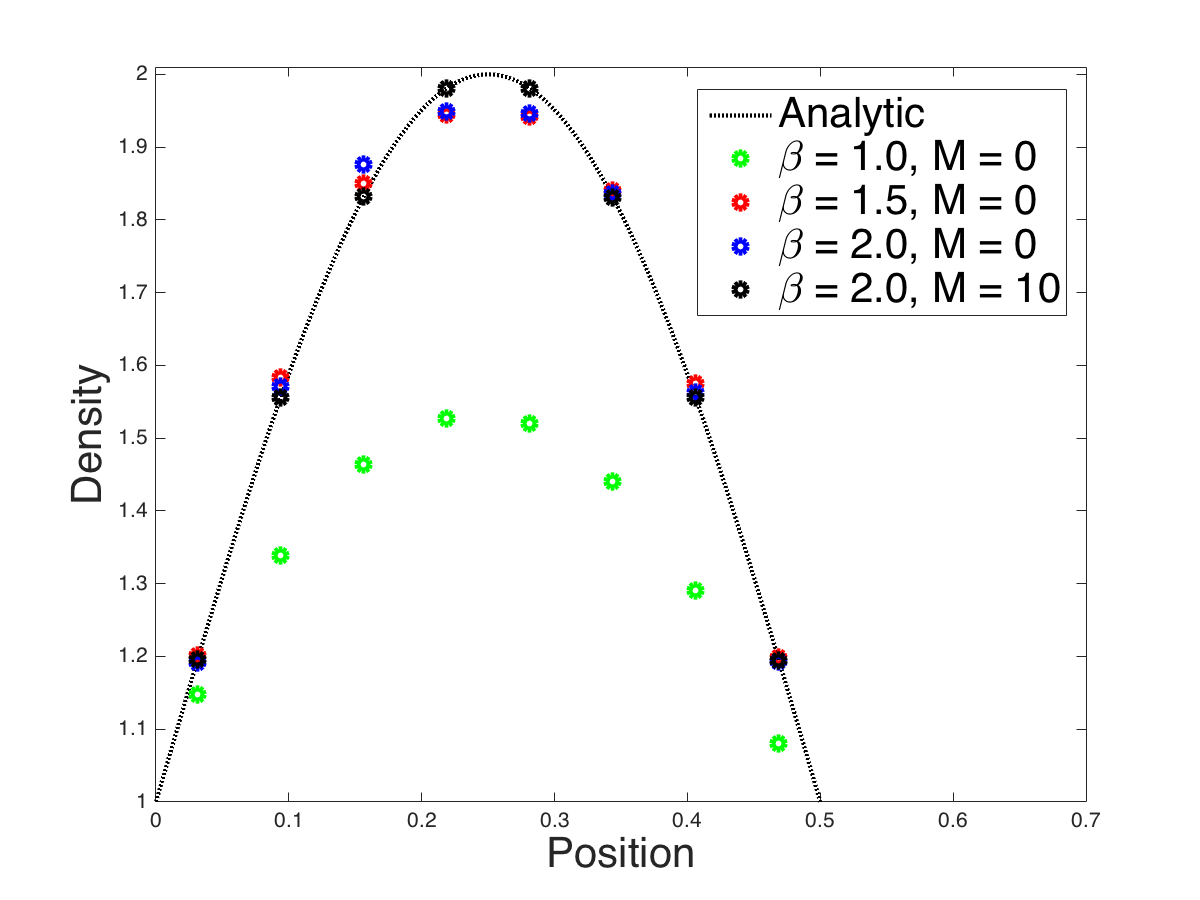
\includegraphics[scale=0.38]{./Figures/StreamingSineWave1D}
  \end{center}
  \caption{Energy density versus position after ten grid crossings ($t=10$) for the streaming sine wave problem computed with the DG(2)+RK3 scheme using 16 elements.  We compare results obtained using various limiter parameters (see text for details) with the analytic solution (dotted line).}
  \label{fig:streamingSineWave}
\end{figure}

\begin{table}
  \begin{center}
  \caption{$L^{\infty}$ error and convergence rates for the streaming sine wave problem.}
  \label{tab:streamingSineWave}
  \begin{tabular}{ccccccccc}
    & \multicolumn{4}{c}{SSP-RK2} & \multicolumn{4}{c}{SSP-RK3} \\
    \cmidrule(r){2-5} \cmidrule(r){6-9}
    $N$ & DG(1) & Rate & DG(2) & Rate & DG(2) & Rate & DG(3) & Rate \\
    \midrule \midrule
    8     & $3.493\times10^{-1}$ & ---  & $9.082\times10^{-3}$ & ---  & $3.310\times10^{-3}$ & ---  & $1.151\times10^{-4}$  & --- \\
    16   & $5.793\times10^{-2}$ &2.59& $2.310\times10^{-3}$ &1.98& $2.652\times10^{-4}$ &3.64& $8.929\times10^{-6}$ &3.69 \\
    32   & $8.423\times10^{-3}$ &2.78& $6.117\times10^{-4}$ &1.92& $3.170\times10^{-5}$ &3.06& $7.911\times10^{-7}$ &3.50 \\
    64   & $1.314\times10^{-3}$ &2.68& $1.574\times10^{-4}$ &1.96& $3.949\times10^{-6}$ &3.00& $7.843\times10^{-8}$ &3.33 \\
    128 & $2.336\times10^{-4}$ &2.49& $3.987\times10^{-5}$ &1.98& $4.934\times10^{-7}$ &3.00& $8.524\times10^{-9}$ &3.20 \\
    256 & $4.736\times10^{-5}$ &2.30& $1.003\times10^{-5}$ &1.99& $6.162\times10^{-8}$ &3.00& $9.997\times10^{-10}$ &3.09 \\
    \midrule \midrule
  \end{tabular}
  \end{center}
\end{table}

\subsection{Spherical Wave}

This problem is taken from \citet{pons_etal_2000}

\begin{figure}
  \begin{center}
    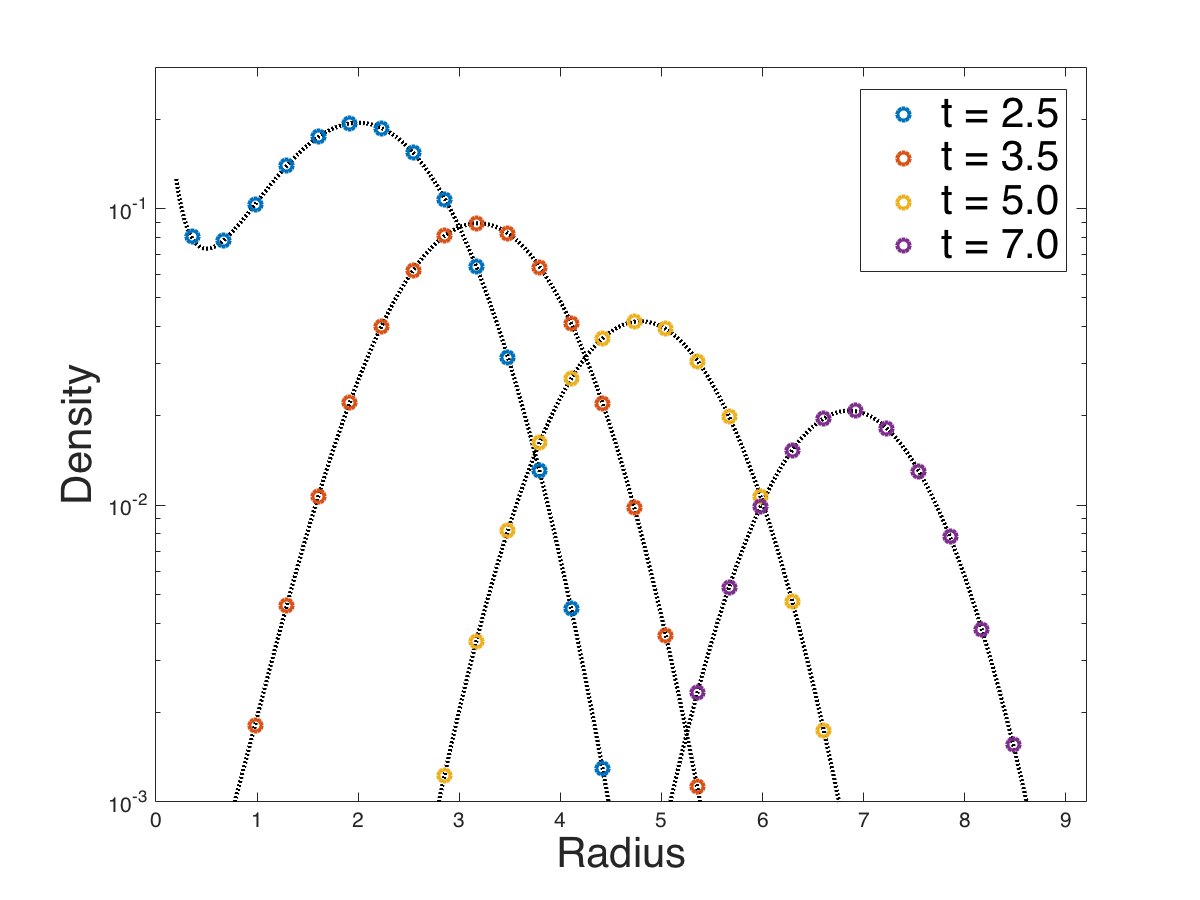
\includegraphics[scale=0.38]{./Figures/GaussianSphericalWave1D}
  \end{center}
  \caption{Energy density versus radius at various times for the spherical wave problem computed with the DG(2)+RK3 scheme using 32 elements.  The numerical solution (open circles) is compared to the analytical solution (dotted lines).  }
  \label{fig:sphericalWave}
\end{figure}

\begin{table}
  \begin{center}
  \caption{$L^{\infty}$ error and convergence rates for the spherical wave problem.}
  \begin{tabular}{ccccccccc}
    & \multicolumn{4}{c}{SSP-RK2} & \multicolumn{4}{c}{SSP-RK3} \\
    \cmidrule(r){2-5} \cmidrule(r){6-9}
    $N$ & DG(1) & Rate & DG(2) & Rate & DG(2) & Rate & DG(3) & Rate \\
    \midrule \midrule
    32   & $4.648\times10^{-4}$ & ---  & $5.540\times10^{-5}$ & ---   & $4.803\times10^{-5}$ & ---  & $1.707\times10^{-5}$ & --- \\
    64   & $9.506\times10^{-5}$ &2.29& $1.088\times10^{-5}$ &2.35& $1.373\times10^{-5}$ &1.81& $7.812\times10^{-7}$ &4.45 \\
    128 & $1.996\times10^{-5}$ &2.25& $1.502\times10^{-6}$ &2.86& $1.836\times10^{-6}$ &2.90& $1.150\times10^{-7}$ &2.76 \\
    256 & $5.783\times10^{-6}$ &1.79& $2.529\times10^{-7}$ &2.57& $1.895\times10^{-7}$ &3.28& $6.268\times10^{-9}$ &4.20 \\
    \midrule \midrule
  \end{tabular}
  \end{center}
\end{table}

\subsection{Line Source}

\subsection{Diffusion Problem}

This problem is adapted from \citet{abdikamalov_etal_2012} \citep[see also][]{pons_etal_2000,sumiyoshiYamada_2012}.  

\begin{equation}
  \cJ(r,t)=\Big(\f{t_{0}}{t_{0}+t}\Big)^{3/2}\,\exp\Big\{\,-\f{3\,\sigma\,r^{2}}{4\,(t_{0}+t)}\,\Big\}
\end{equation}

\begin{figure}
  \begin{center}
    \begin{tabular}{cc}
      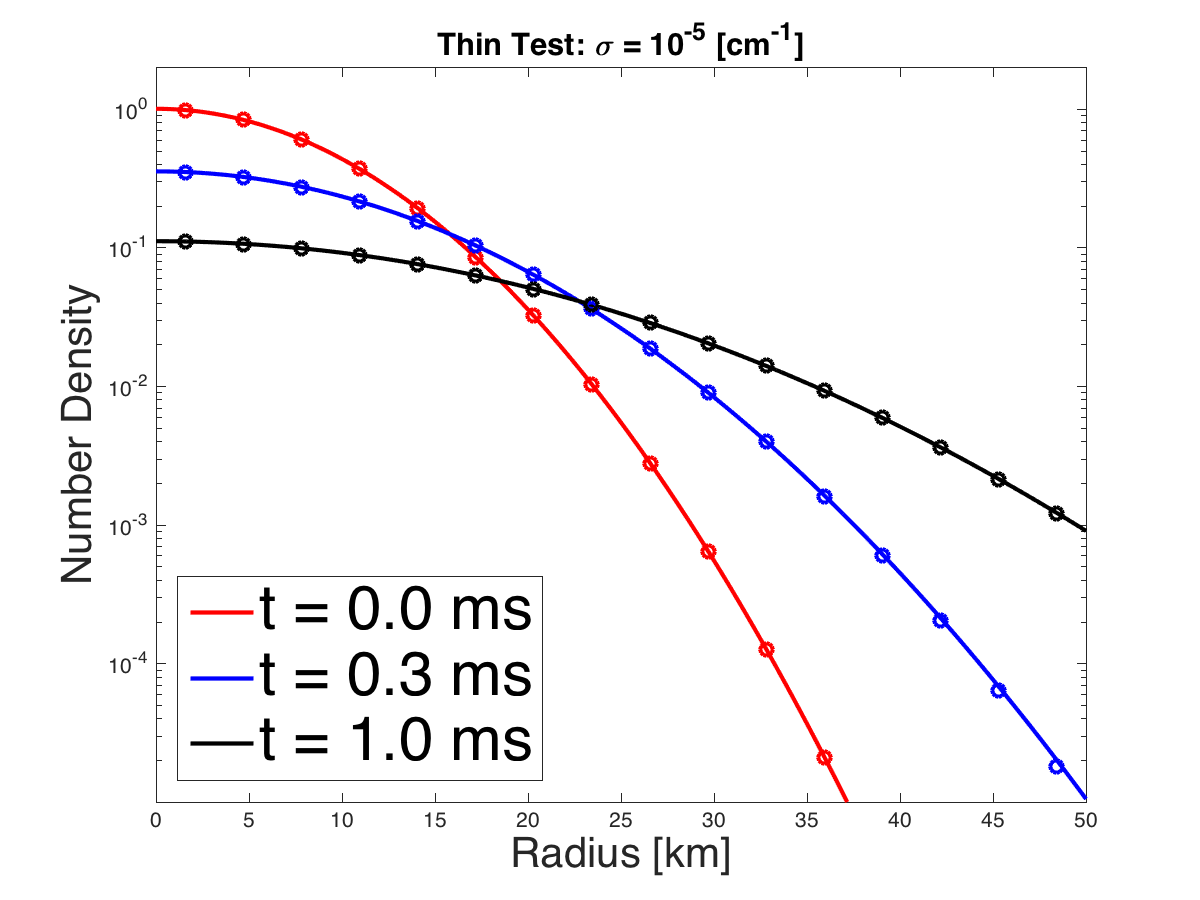
\includegraphics[scale=0.38]{./Figures/GaussianSphericalDiffusion_Kappa_1e-5_Density} &
      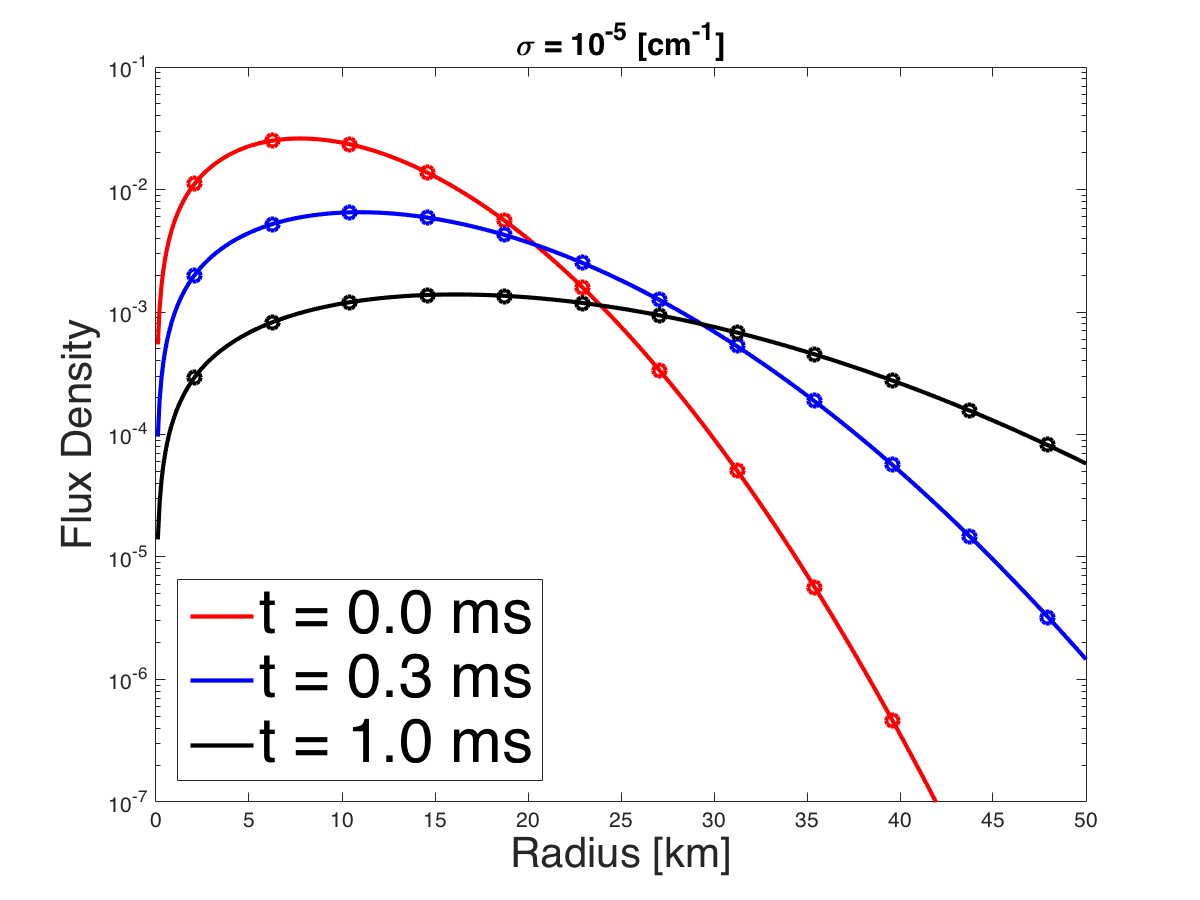
\includegraphics[scale=0.38]{./Figures/GaussianSphericalDiffusion_Kappa_1e-5_Flux}
    \end{tabular}
  \end{center}
  \caption{Results from the one-dimensional diffusion problem in spherical symmetry with $\sigma=10^{-5}$~cm$^{-1}$, obtained with the DG(2)+SIRK2 method using $24$ elements.  
  The number density $\cJ$ (left panel) and the number flux density $\cH_{r}$ (right panel) are plotted for $t=0,0.3,1.0$~ms (red, blue, and black curves, respectively).  
  Solid lines represent the analytical solution while open circles represent the element center value of the numerical solution.}
  \label{fig:diffusionProblem1e-5}
\end{figure}

\begin{figure}
  \begin{center}
    \begin{tabular}{cc}
      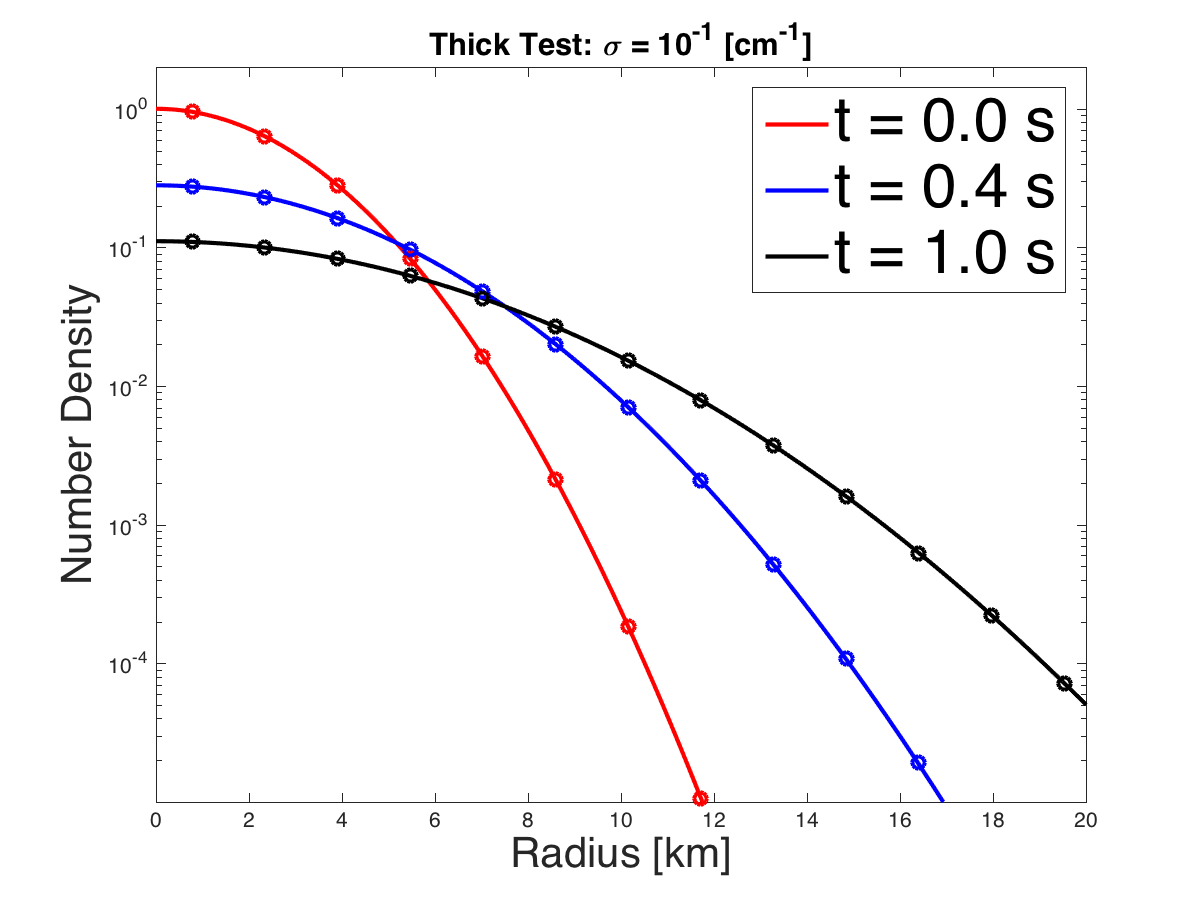
\includegraphics[scale=0.38]{./Figures/GaussianSphericalDiffusion_Kappa_1e-1_Density} &
      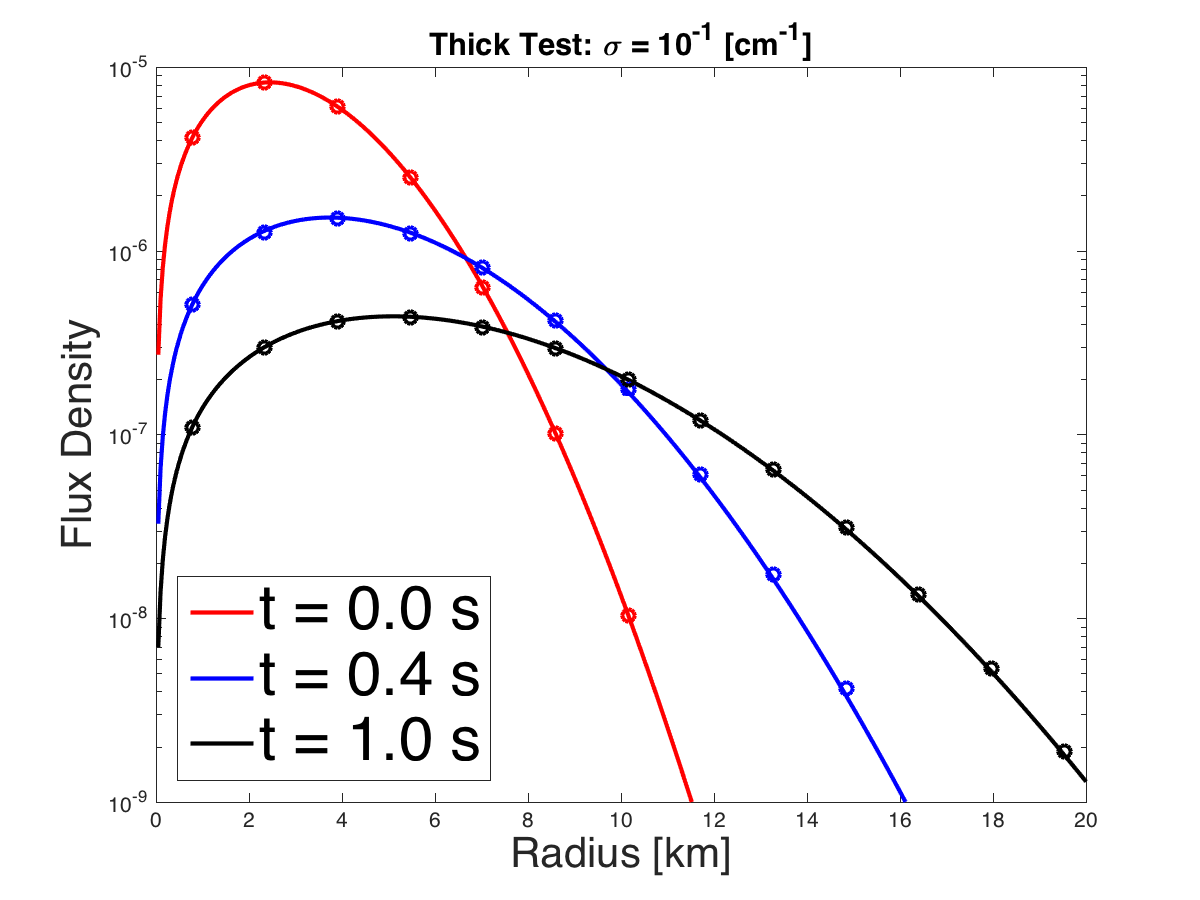
\includegraphics[scale=0.38]{./Figures/GaussianSphericalDiffusion_Kappa_1e-1_Flux}
    \end{tabular}
  \end{center}
  \caption{Results similar to those displayed in Figure~\ref{fig:diffusionProblem1e-5}, but with $\sigma=10^{-1}$~cm$^{-1}$.}
  \label{fig:diffusionProblem1e-1}
\end{figure}

\subsection{Homogeneous Sphere}

\bibliographystyle{apj}
\bibliography{../References/references.bib}

\appendix

\section{Moment Equations in Commonly Used Coordinate Systems}
\label{app:CurvilinearEuler}

\subsection{Cylindrical Coordinates}

\begin{equation}
  \pderiv{\cJ}{t}
  +\f{1}{R}\pderiv{}{R}\Big(R\,\cH_{R}\Big)
  +\pderiv{}{z}\Big(\cH_{z}\Big)
  +\f{1}{R}\pderiv{}{\phi}\Big(\cH_{\phi}\Big)=0,
\end{equation}
\begin{equation}
  \pderiv{\big(\rho\,v_{R}\big)}{t}
  +\f{1}{R}\pderiv{}{R}\Big(R\,\big(\rho\,v_{R}\,v_{R}+p\big)\Big)
  +\pderiv{}{z}\Big(\rho\,v_{R}\,v_{z}\Big)
  +\f{1}{R}\pderiv{}{\phi}\Big(\rho\,v_{R}\,v_{\phi}\Big)
  =\f{\big(\rho\,v_{\phi}^{2}+p\big)}{R},
\end{equation}
\begin{equation}
  \pderiv{\big(\rho\,v_{z}\big)}{t}
  +\f{1}{R}\pderiv{}{R}\Big(R\,\rho\,v_{z}\,v_{R}\Big)
  +\pderiv{}{z}\Big(\big(\rho\,v_{z}\,v_{z}+p\big)\Big)
  +\f{1}{R}\pderiv{}{\phi}\Big(\rho\,v_{z}\,v_{\phi}\Big)=0,
\end{equation}
\begin{equation}
  \pderiv{\big(\rho\,v_{\phi}\big)}{t}
  +\f{1}{R}\pderiv{}{R}\Big(R\,\rho\,v_{\phi}\,v_{R}\Big)
  +\pderiv{}{z}\Big(\rho\,v_{\phi}\,v_{z}\Big)
  +\f{1}{R}\pderiv{}{\phi}\Big(\rho\,v_{\phi}\,v_{\phi}+p\Big)
  =-\f{\rho\,v_{\phi}\,v_{R}}{R},
\end{equation}

\subsection{Spherical Coordinates}

\begin{equation}
  \pderiv{\rho}{t}
  +\f{1}{r^{2}}\pderiv{}{r}\Big(r^{2}\,\rho\,v_{r}\Big)
  +\f{1}{r\sin\theta}\pderiv{}{\theta}\Big(\sin\theta\,\rho\,v_{\theta}\Big)
  +\f{1}{r\sin\theta}\pderiv{}{\phi}\Big(\rho\,v_{\phi}\Big)=0,
\end{equation}
\begin{equation}
  \pderiv{\big(\rho\,v_{r}\big)}{t}
  +\f{1}{r^{2}}\pderiv{}{r}\Big(r^{2}\,\big(\rho\,v_{r}\,v_{r}+p\big)\Big)
  +\f{1}{r\sin\theta}\pderiv{}{\theta}\Big(\sin\theta\,\rho\,v_{r}\,v_{\theta}\Big)
  +\f{1}{r\sin\theta}\pderiv{}{\phi}\Big(\rho\,v_{r}\,v_{\phi}\Big)
  =\rho\,\f{\big(v_{\theta}^{2}+v_{\phi}^{2}\big)}{r}+\f{2\,p}{r},
\end{equation}
\begin{equation}
  \pderiv{\big(\rho\,v_{\theta}\big)}{t}
  +\f{1}{r^{2}}\pderiv{}{r}\Big(r^{2}\,\rho\,v_{\theta}\,v_{r}\Big)
  +\f{1}{r\sin\theta}\pderiv{}{\theta}\Big(\sin\theta\,\big(\rho\,v_{\theta}\,v_{\theta}+p\big)\Big)
  +\f{1}{r\sin\theta}\pderiv{}{\phi}\Big(\rho\,v_{\theta}\,v_{\phi}\Big)
  =\cot\theta\,\f{\big(\rho\,v_{\phi}^{2}+p\big)}{r}-\rho\,\f{v_{r}\,v_{\theta}}{r},
\end{equation}
\begin{equation}
  \pderiv{\big(\rho\,v_{\phi}\big)}{t}
  +\f{1}{r^{2}}\pderiv{}{r}\Big(\,r^{2}\,\rho\,v_{\phi}\,v_{r}\,\Big)
  +\f{1}{r\sin\theta}\pderiv{}{\theta}\Big(\sin\theta\,\rho\,v_{\phi}\,v_{\theta}\Big)
  +\f{1}{r\sin\theta}\pderiv{}{\phi}\Big(\rho\,v_{\phi}\,v_{\phi}+p\Big)
  =-\rho\,v_{\phi}\,\f{\big(v_{r}+v_{\theta}\,\cot\theta\big)}{r},
\end{equation}

\end{document}